% Figure s02f02_cosband (Session 2): the one-dimensional band and its density of states.
% The image is rendered by figures/blender/s02f02_cosband.py; the coordinates of the labels come from
% figures/blender/out/s02f02_cosband_anchors.tex. Build with figures/blender/build_figure.sh s02f02_cosband.
\documentclass[11pt,tikz,border=0pt]{standalone}
\usepackage[T1]{fontenc}
\usepackage{amsmath,amssymb,graphicx,bm}
\usepackage{xcolor}
\usetikzlibrary{arrows.meta,calc}
% The three label colors of the figures, with the same values as in src/figures_preamble.tex.
\definecolor{aqmaccent}{RGB}{31,78,121}
\definecolor{aqmbroken}{RGB}{168,42,34}
\definecolor{aqmmuted}{RGB}{125,125,125}

\newlength{\figw}\setlength{\figw}{15.6cm}   % the text width of the notes (A4, 2.7 cm margins)

\begin{document}
\begin{tikzpicture}[lbl/.style={font=\small, inner sep=1.5pt}, pnl/.style={font=\small\bfseries, inner sep=1.5pt}]
  \node[anchor=south west, inner sep=0pt] at (0,0)
    {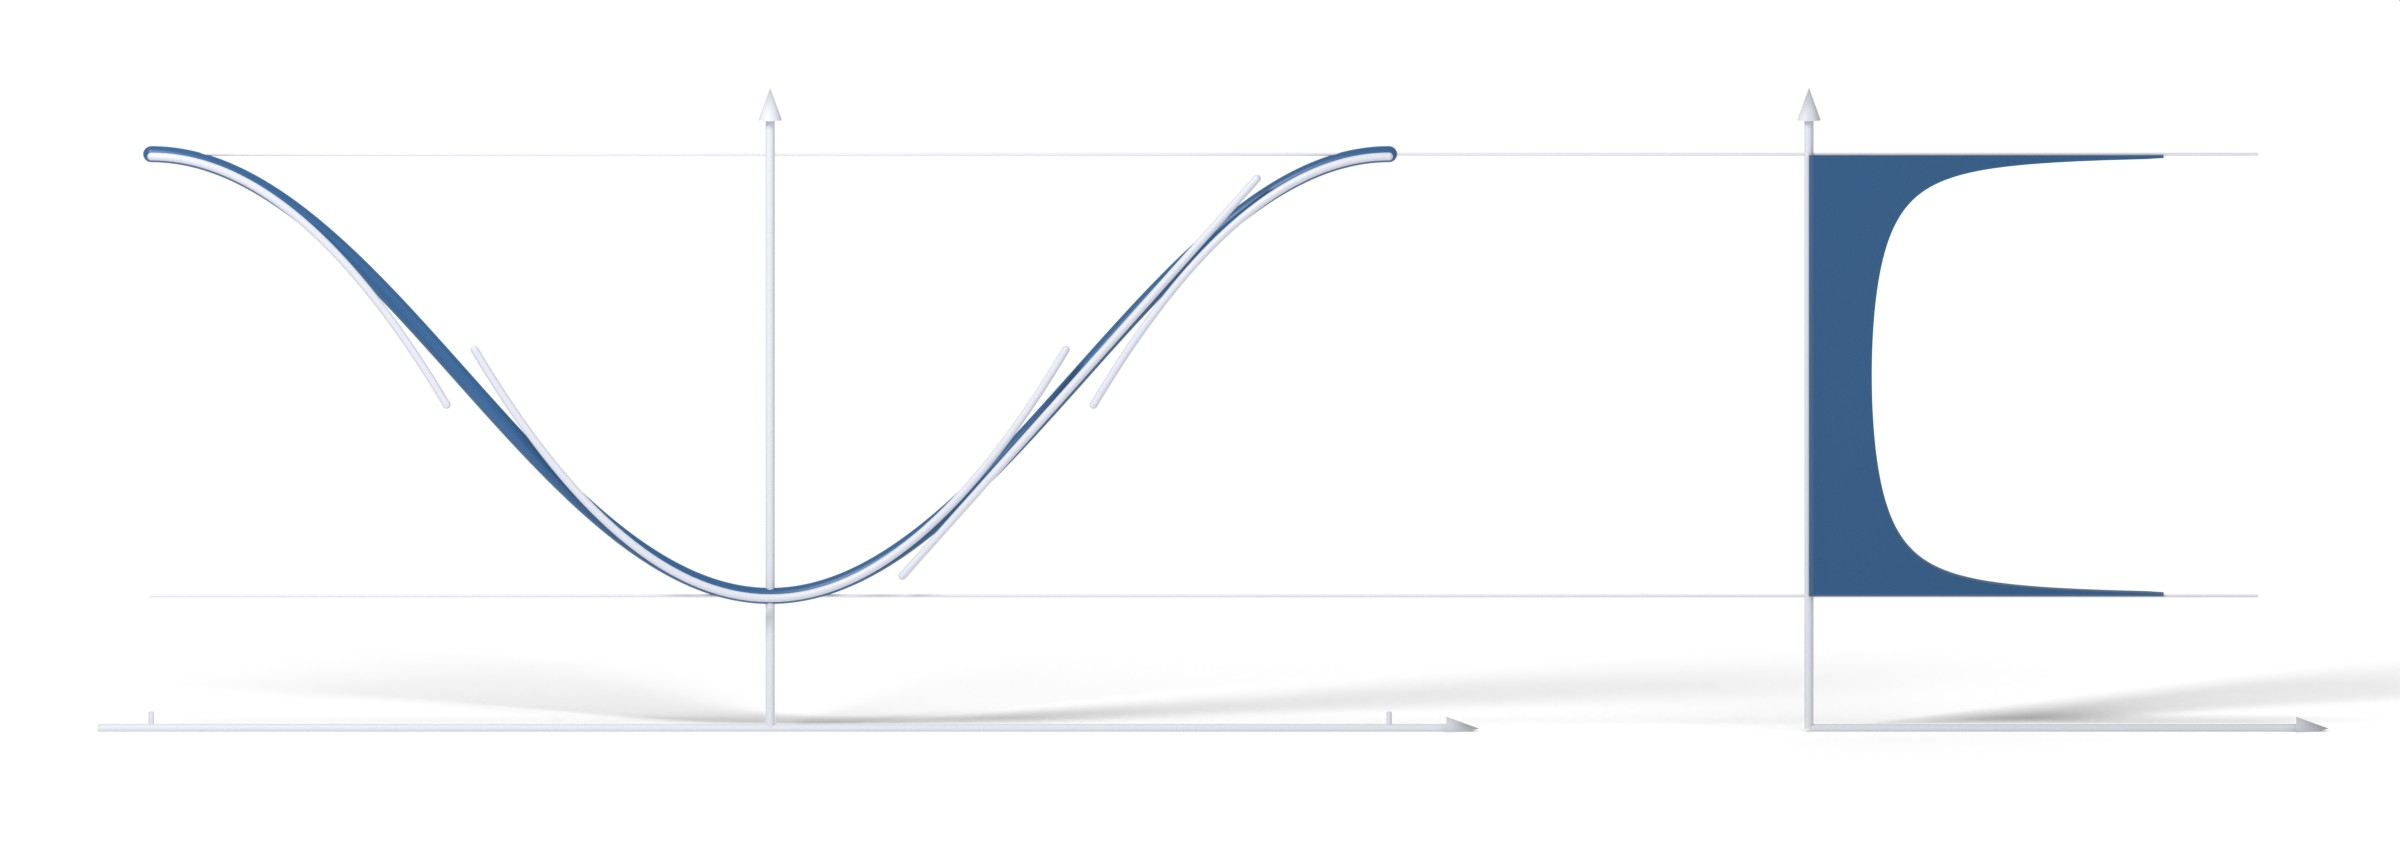
\includegraphics[width=\figw]{../blender/out/s02f02_cosband.jpg}};
  %% written by figlib.py; x and y in units of the image width
\coordinate (mpi) at (0.0630\figw,0.0513\figw);
\coordinate (zero) at (0.3209\figw,0.0513\figw);
\coordinate (pi) at (0.5788\figw,0.0513\figw);
\coordinate (phi) at (0.6161\figw,0.0536\figw);
\coordinate (E) at (0.3209\figw,0.3204\figw);
\coordinate (bottom) at (0.3209\figw,0.1033\figw);
\coordinate (top) at (0.5788\figw,0.2984\figw);
\coordinate (mid) at (0.4646\figw,0.1847\figw);
\coordinate (E2) at (0.7537\figw,0.3204\figw);
\coordinate (g) at (0.9701\figw,0.0536\figw);
\coordinate (peak) at (0.9052\figw,0.2859\figw);
\coordinate (m2t) at (0.7537\figw,0.1088\figw);
\coordinate (p2t) at (0.7537\figw,0.2928\figw);

  \node[lbl, anchor=north] at (mpi) {$-\pi$};
  \node[lbl, anchor=north] at (zero) {$0$};
  \node[lbl, anchor=north] at (pi) {$\pi$};
  \node[lbl, anchor=west] at (phi) {$\varphi$};
  \node[lbl, anchor=south] at (E) {$\epsilon_\varphi$};
  \node[lbl, anchor=north] at (bottom) {parabola, electrons with positive mass};
  \node[lbl, anchor=south east] at (top) {inverted parabola, holes};
  \node[lbl, anchor=west, align=left] at (mid) {linear, the slope\\is the group velocity};
  \node[lbl, anchor=south] at (E2) {$\epsilon$};
  \node[lbl, anchor=south east] at (g) {$g(\epsilon)$};
  \node[lbl, anchor=east] at (m2t) {$-2t$};
  \node[lbl, anchor=east] at (p2t) {$2t$};
\end{tikzpicture}
\end{document}
